% Ubah judul dan label berikut sesuai dengan yang diinginkan.
\section{Arsitektur}
\label{sec:arsitektur}

% Ubah paragraf-paragraf pada bagian ini sesuai dengan yang diinginkan.

\subsection{Retriever}
\label{subsec:Retriever}

Sebelum menggunakan data untuk model bahasa, perlu dilakukan pencarian data yang relevan. Untuk melakukan pencarian data ini, dilakukan pencarian dengan melihat lokasi data dalam vektor. Untuk itu perlu mengubah data menjadi bentuk vektor yang dapat dihitung. Ada banyak metode untuk melakukan ini, seperti \emph{one-hot}, \emph{Word2Vec}, dan \emph{Doc2Vec}. Metode-metode ini menyediakan jalur efektif untuk kuantifikasi teks tetapi seringkali mengabaikan informasi kontekstual. Model \emph{Transformer}, yang diperkenalkan oleh Google pada tahun 2017, mengatasi kekurangan metode kuantifikasi teks yang ada dan dibangun menggunakan pelatihan tanpa pengawasan pada volume besar data korpus yang tidak berlabel \cite{vaswani2017attention}. \emph{Transformer} adalah arsitektur jaringan saraf yang banyak digunakan dalam NLP, klasifikasi teks, sistem tanya jawab, dan lainnya. Model ini terdiri dari beberapa \emph{encoder} dan \emph{decoder}, yang masing-masing terdiri dari beberapa lapisan blok identik. Blok-blok ini ditumpuk bersama untuk membentuk arsitektur keseluruhan \emph{Transformer} \cite{miao2016processing}. Struktur dari \emph{transformer} dapat dilihat pada Gambar \ref*{fig:transformer}
\begin{figure*}
  \centering
  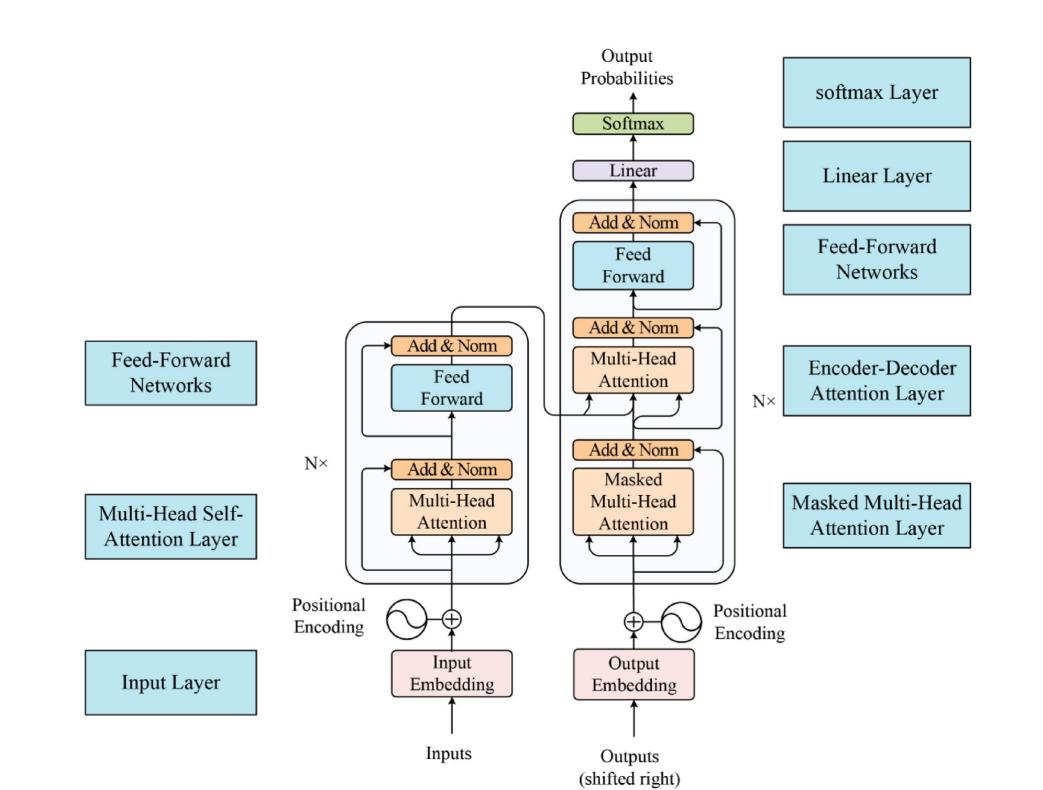
\includegraphics[width=.7\textwidth]{gambar/struktur-transformer.jpg}
  \caption{Struktur \emph{transformer} \cite{vaswani2017attention}}
  \label{fig:transformer}
\end{figure*}

Dalam arsitektur \emph{transformer}, terdapat dua komponen utama yaitu \emph{encoder} dan \emph{decoder}, masing-masing terdiri dari serangkaian lapisan yang sama. Setiap lapisan dalam \emph{encoder} dan \emph{decoder} memiliki dua sub-lapisan, yaitu mekanisme \emph{multi-head attention} dan \emph{fully connected network}. \emph{Multi-head attention}memungkinkan model untuk memproses bagian-bagian dari data secara paralel dan mengintegrasikan informasi dari berbagai posisi dalam data. Selain itu, \emph{transformer} memiliki mekanisme \emph{self-attention}, yang memungkinkan setiap output dari \emph{encoder} atau \emph{decoder} untuk mempertimbangkan seluruh input sebelumnya. Hal ini berbeda dengan algoritma-algoritma lain yang terbatas oleh jarak antara input yang relevan dan output. Mekanisme ini juga membantu dalam memahami dependensi jangka panjang dalam teks, yang sangat penting untuk tugas-tugas seperti penerjemahan. \emph{Positional encoding} digunakan untuk memberikan informasi posisi kepada model, karena model \emph{transformer} tidak memiliki rekurensi atau konvolusi yang secara alami menangkap urutan informasi \cite{vaswani2017attention}. 

\subsection{Augment dan Generation}
\label{subsec:AugmentGeneration}

Pada proses \emph{augmentation}, model LLM akan bekerja dengan memproses \emph{prompt} dari pengguna dengan menggunakan konteks yang sudah diperoleh dari proses \emph{retriever} sebelumnya \cite{bansal2024llm}. Alat diimplementasikan dengan pertama-tama membuat sistem backend menggunakan LangChain untuk menghubungkan berbagai modul dan proses LLM. LangChain berfungsi sebagai penghubung dengan berbagai modul lainnya. Selanjutnya dilakukan pemilihan framework LLM yang akan digunakan. Framework yang digunakan harus bersifat \emph{open-source} dan ringan agar dapat efektif dalam penggunaan. Oleh karena itu, dalam tahapan pengujian, akan dilakukan uji coba pada berbagai framework untuk menguji efektivitas dari framework-framework tersebut. Beberapa yang akan diujikan adalah RASA, Hugging Face, dan Ilama Cpp. Pengujian dilakukan dengan melihat kinerja masing-masing framework, serta mempertimbangkan kelebihan dan kekurangan mereka. Setelah itu, akan dipilih framework yang paling efektif untuk digunakan dalam implementasi alat ini.

Pada proses \emph{generation}, model LLM akan menghasilkan output berupa jawaban dari pertanyaan yang diberikan oleh pengguna. Output ini akan diberikan kepada pengguna sebagai jawaban dari pertanyaan yang diberikan. Dalam proses ini, model LLM akan menggunakan konteks yang sudah diperoleh dari proses \emph{retriever} sebelumnya. Dengan demikian, model LLM akan dapat memberikan jawaban yang lebih relevan dan akurat. Dalam pengetesan digunakan konfigurasi sebagai berikut:

\begin{lstlisting}[
  language=python,
  caption={Konfigurasi tes},
]
model = AutoModelForCausalLM.from_pretrained(
   "$MODEL_NAME",
    device_map='auto',
    load_in_8bit=True,
    trust_remote_code=True)

pipeline = pipeline(
    "text-generation",
    model=model,
    return_full_text=False,
    tokenizer=tokenizer,
    max_new_tokens=512,
     do_sample=True,
    pad_token_id=tokenizer.eos_token_id
)
\end{lstlisting}

Setelah itu, dilakukan analisa terhadap hasil yang diperoleh dari model LLM. Hasil yang diperoleh akan dianalisa berdasarkan relevansi dan akurasi jawaban yang diberikan. Hal ini dilakukan dengan membandingkan jawaban dengan jawaban pada sumber data. Sebagai contoh, untuk pertanyaan: "Apa yang harus dilakukan jika terjadi pemadaman listrik?"  maka jawaban yang relevan sesuai buku adalah "Jika terjadi pemadaman listrik, jangan panik, generator darurat akan memulihkan daya dalam waktu sigkat, cari tahu masalah dan alasan pemadaman listrik, informasikan kepada petugas...". Selain itu, dilakukan analisa terhadap penggunaan RAM dan VRAM. Hal ini dilakukan untuk mengetahui seberapa efisien model LLM dalam penggunaan sumber daya. Dengan demikian, dapat diketahui seberapa efektif model LLM dalam memberikan jawaban yang relevan, akurat, dan efektif.

% Contoh input gambar pada kolom.
% \begin{figure} [ht]
%   \centering
%   % Ubah sesuai dengan nama file gambar dan ukuran yang akan digunakan.
%   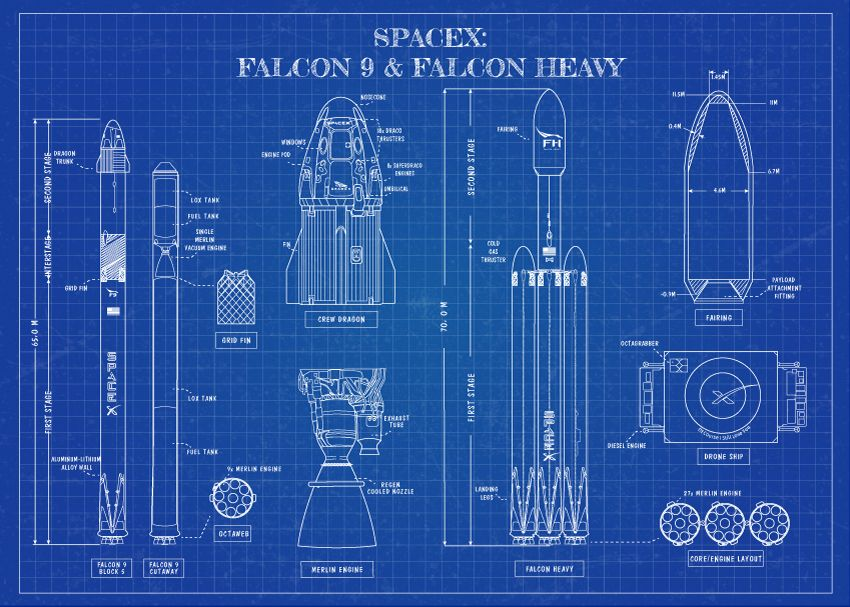
\includegraphics[width=0.4\textwidth]{gambar/cetakbiru.jpg}

%   % Ubah sesuai dengan keterangan gambar yang diinginkan.
%   \caption{Cetak biru roket yang akan diuji coba. \cite{cetakbiruspacex}}
%   \label{fig:cetakbiru}
% \end{figure}

% \lipsum[9-10]

% \subsection{Lorem Ipsum}
% \label{subsec:loremipsum}

% \lipsum[11]

% % Contoh pembuatan tabel.
% \begin{table}
%   \caption{Contoh tabel sederhana}
%   \label{tab:tabelsederhana}
%   \centering
%   \begin{tabular}{lll}
%     \toprule
%     Heading1 & Heading2 & Heading3  \\
%     \midrule
%     One      & Two      & Three     \\
%     Four     & Five     & Six       \\
%     \bottomrule
%   \end{tabular}
% \end{table}

% % Contoh pembuatan potongan kode.
% \begin{lstlisting}[
%   language=C++,
%   caption={Program halo dunia.},
%   label={lst:halodunia}
% ]
% #include <iostream>

% int main() {
%     std::cout << "Halo Dunia!";
%     return 0;
% }
% \end{lstlisting}

% \lipsum[12]

% % Contoh pembuatan daftar.
% \begin{enumerate}
%   \item \lipsum[13][1-4]
%   \item \lipsum[13][5-8]
%   \item \lipsum[13][9-12]
% \end{enumerate}

% \lipsum[14-15]
